\chapter{General Context}
\label{ch:context}
\minitoc

\section*{Introduction}
\addcontentsline{toc}{section}{Introduction}
This Chapter sets out where the project came from and what it was asked to solve. It introduces the institution that hosted the work and the client whose document sits at the center of it, then looks closely at how the document is used today. That second part carries more weight than it might appear: The requirements at the end of this chapter are not invented, they are what is left once you understand exactly how the current process fails. The chapter closes with the tools that already exist for this kind of problem, why none of them fit, and the solution proposed in response.

\section{General Framework of the Project}
This was a Final Year Project (FYP) inside the master's degree program in Data Sciences at Polytech Intl, carried out over a six months internship. Roughly four of those months went into building the system. The rest went on framing the subject, learning the source material well enough to be useful, and writing the report.



 What kept me on this was how ordinary the document looks and how badly it breaks automated tools. A person reads a page of the DAM without difficulty. Every library I pointed at the same page came back with something plausible and wrong, and finding out why meant learning to read the file the way the printer wrote it rather than the way a reader sees it. 
 
Table~\ref{tab:framework} summarises the arrangement.
\begin{table}[h]
\centering
\caption{Framework of the project.}
\label{tab:framework}
\begin{tabular}{|p{0.34\textwidth}|p{0.56\textwidth}|}
\hline
\rowcolor{myblue}\textcolor{white}{\textbf{Item}} & \textcolor{white}{\textbf{Detail}} \\
\hline
Project type & End-of-studies project \\ \hline
Host institution & Polytech Intl, Tunis \\ \hline
Programme & Professional Master's in Data Science \\ \hline
Academic year & 2025 -- 2026 \\ \hline
Duration & Six months \\ \hline
Client organisation & African Development Bank Group \\ \hline
Academic supervisor & Dr.~Marouene Chaieb \\ \hline
Professional supervisors & Mr.~Yasser Ahmad, Mr.~Surya Joymungul \\ \hline
Source document & Delegation of Authority Matrix, over 250 pages \\ \hline
Scope processed & 79-page subset covering three chapters \\ \hline
\end{tabular}
\end{table}
\section{Host Organisation}
\label{sec:hostorg}

Two institutions were involved in this project, with different parts to play. Polytech
Intl provided the academic framework: the supervision, and the requirements the work had
to satisfy as a degree project. The African Development Bank provided the document at the
centre of the work, along with the operational judgement of whether an answer the system
produced would be trusted by someone who had to act on it. A university could not have
supplied the second of those, and a bank could not have supplied the first. The
subsections below introduce each in turn.

\subsection{Presentation of Polytech Intl}


Polytech Intl \citep{polytechintl}, the \'Ecole Polytechnique Internationale Priv\'ee de Tunis, is a
private higher education institution founded in 2013 and based at Rue du Lac
d'Annecy in Les Berges du Lac~1, Tunis. It was set up largely by institutional
figures from the professional world, principally from banking, insurance and
industry, which is visible in how the school approaches training: the intent is
that graduates leave employable, and ideally capable of building something of
their own.

Teaching covers engineering and related disciplines. Programmes run across
computer science, with tracks in big data, business intelligence, software
engineering, IT-finance and embedded systems, alongside mechatronics, industrial
engineering, financial engineering, telecommunications and architecture.
Students are also offered international mobility, with internships and teaching
modules arranged in partnership with schools in Europe, Asia and North America.
The school is a member of the Agence Universitaire de la Francophonie.

The Data Sciences Master's spans statistics and machine learning, data
engineering, and the software side of turning an analysis into something that
runs and keeps running. A final project is meant to show all three. That
expectation is part of why this one was pushed through to a deployed application
instead of stopping at a clean dataset.

\subsection{Project Context and the Client Organisation}

Polytech Intl hosted and supervised the project. The subject came from elsewhere.
The document at the centre of it belongs to the African Development Bank Group \citep{afdb},
which acted as the client. There is a certain symmetry in that: a school founded
in part by people from banking, supervising a project built for a bank.

The African Development Bank Group was founded in 1964 \citep{afdb} and has its headquarters
in Abidjan, C\^ote d'Ivoire. Eighty-one countries are members, 54 of them
African and 27 from outside the continent, and the Bank exists to support
economic development and social progress across its regional member countries.
Table~\ref{tab:afdb} sets out the essentials.

\begin{table}[h]
\centering
\caption{Client organisation at a glance.}
\label{tab:afdb}
\begin{tabular}{|p{0.34\textwidth}|p{0.56\textwidth}|}
\hline
\rowcolor{myblue}\textcolor{white}{\textbf{Item}} & \textcolor{white}{\textbf{Detail}} \\
\hline
Institution & African Development Bank Group \\ \hline
Founded & 1964 \\ \hline
Headquarters & Abidjan, C\^ote d'Ivoire \\ \hline
Membership & 81 countries: 54 regional, 27 non-regional \\ \hline
Purpose & Economic development and social progress across regional member countries \\ \hline
Group entities & African Development Bank, African Development Fund, Nigeria Trust Fund \\ \hline
Regional office concerned & RDGN: Tunisia, Algeria, Morocco, Mauritania, Libya \\ \hline
Regional hub & Tunis \\ \hline
\end{tabular}
\end{table}

Working from a real institution's document changed how the project had to be
done. The material could not be tidied up to suit the parser. Correctness meant
whatever the printed pages say, not a score that happened to be easy to compute.
And every claim in this report about what the system pulls out of the document
can be checked against the page it came from. That constraint runs through the
whole of Chapter~2.

\section{Study of the Existing System and Critical Analysis}

The point of this section is to stress that one cannot judge the adequacy of the tools we have until we know what adequacy means in this instance. Section~\ref{sec:damcontext} details the requirements the document places on its users, while Section~\ref{sec:existingsystems} compares the resources currently available against those requirements. This suggests there is an argument in this section, not just content.

\subsection{Context of Delegation of Authority in Development Banking}
\label{sec:damcontext}

Before the document's shortcomings can be assessed, it has to be described on its own
terms: what it is for, how its notation works, and what happens when that notation is
misread.

\subsubsection{Definition and Stakes of the DAM}

The Delegation of Authority Matrix (DAM) is an internal Bank document \citep{afdb_dam} that sets out who is responsible for taking specific actions on identified tasks. The Task Managers of the African Development Bank depend on it to delegate the authority of the President down to the appropriate level for a decision to be made. Without it, every decision would require the President's approval.

A DAM page consists of two tables that fill the page, as shown in Figure~\ref{fig:DamPage}. The bottom of each page is reserved for footnotes. A brief reminder of what the letters in the authority codes mean is printed in the upper right, but it only goes so far: it explains the letters and not the numbers that qualify them. The main table carries the process, the sub-task, and the roles with their assigned authority codes.

\begin{figure}[htbp]
    \centering
    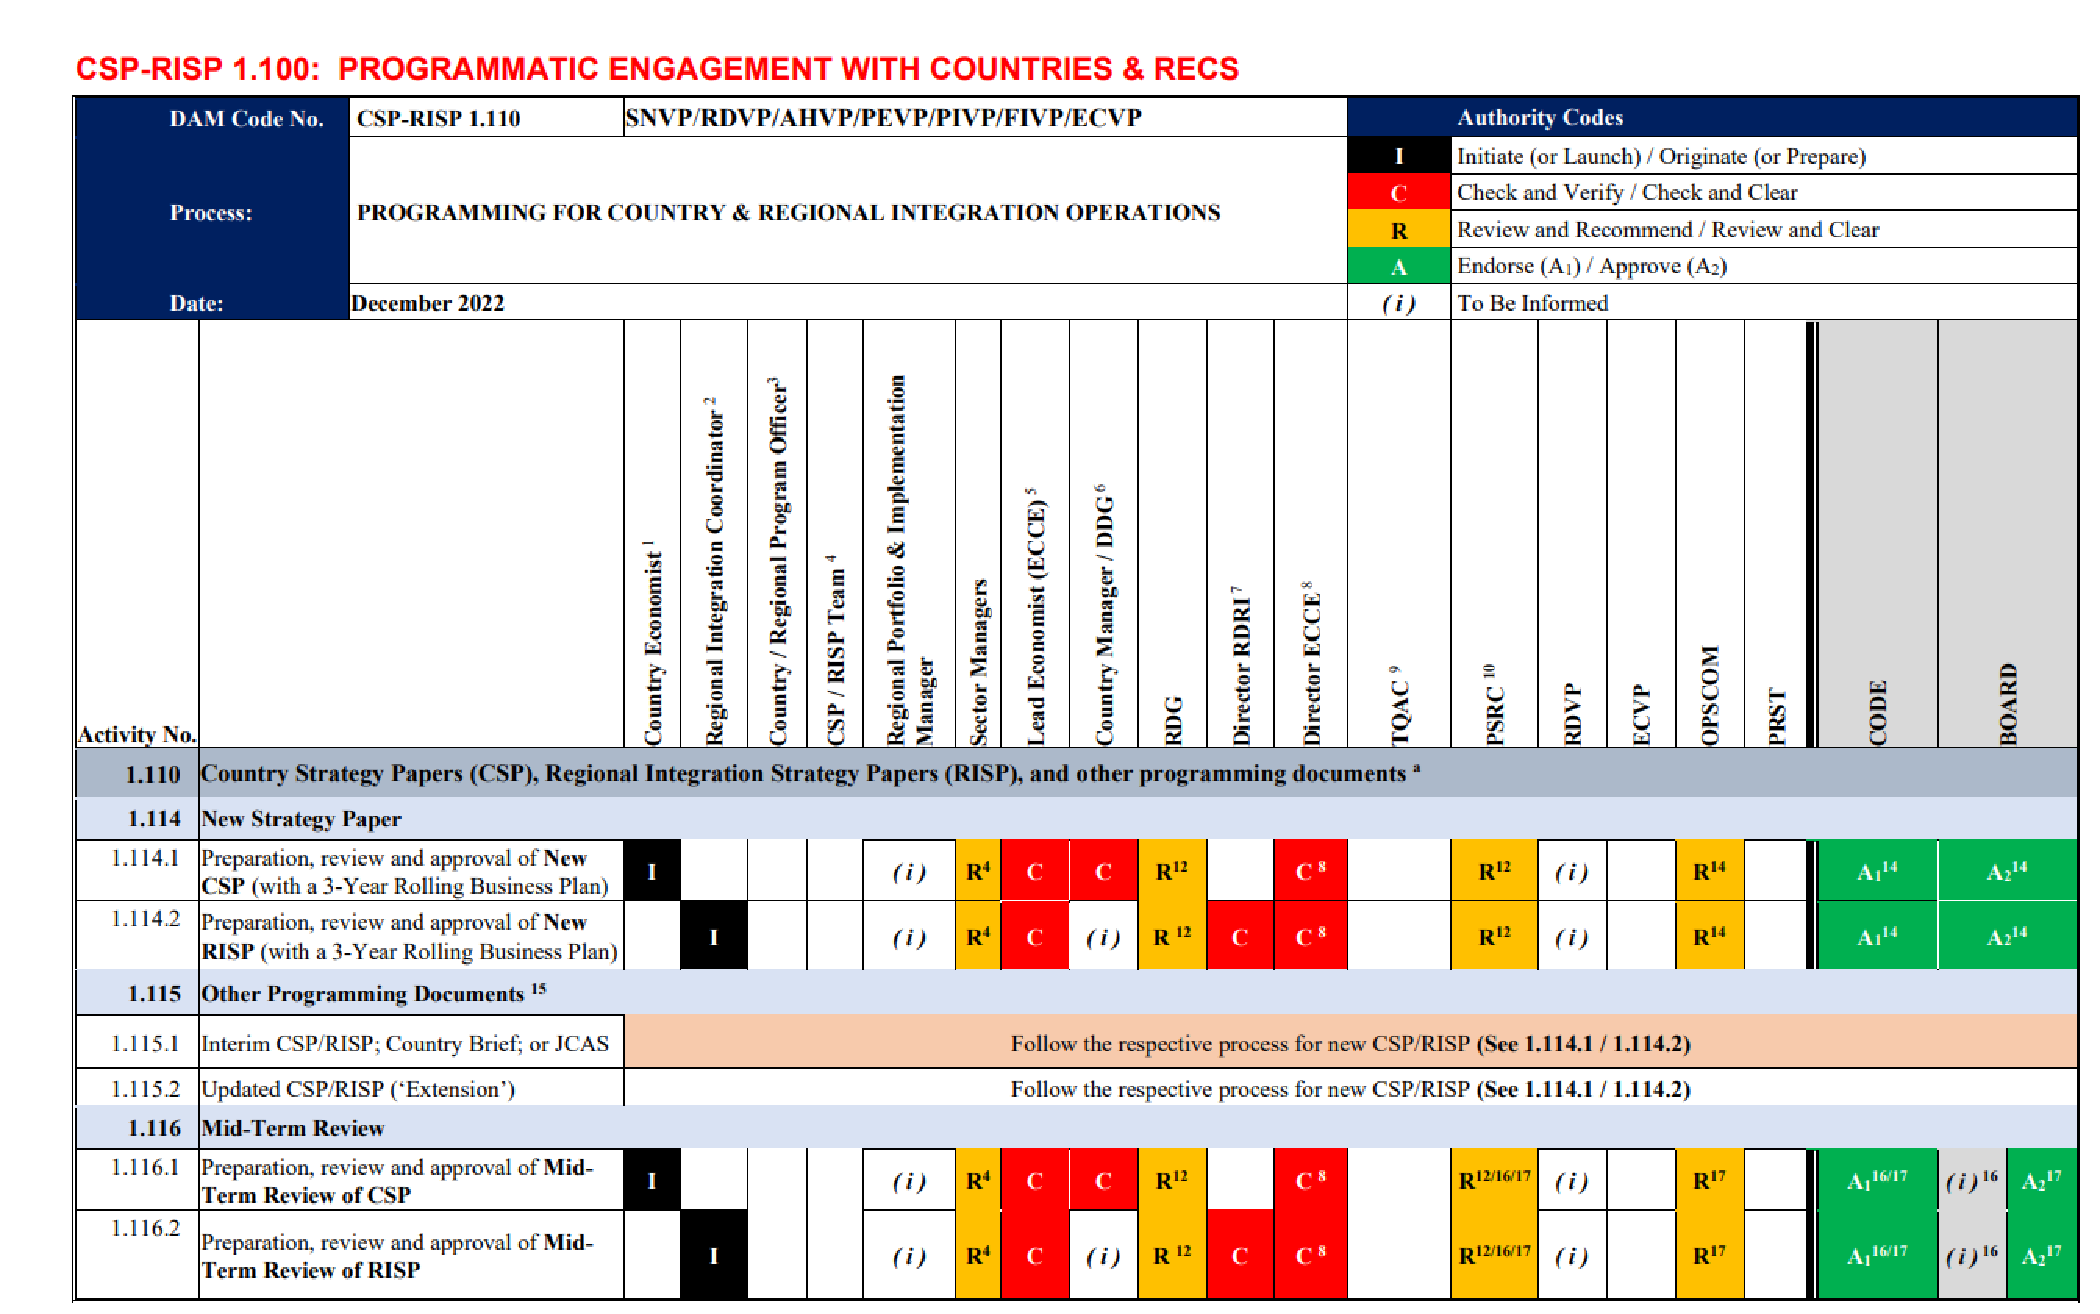
\includegraphics[width=0.88\linewidth]{figures/Capture d'écran 2026-09-16 184640.pdf}
    \caption{Example of a DAM page, showing the two stacked tables and the footnote band at the foot of the page.}
    \label{fig:DamPage}
\end{figure}

There are five authority codes but seventeen distinct notations, because most codes take a level, and the letter alone is therefore not the answer. Take C: on its own it denotes Check and Verify, and C1 and C2 are its two levels:

\begin{itemize}
\item \textbf{C1} --- examine the activity against a checklist of standards and preconditions, and allow it to proceed only if all of them are satisfied.
\item \textbf{C2} --- clear the activity as compliant with policy and regulation, after consulting the relevant departments.
\end{itemize}

Both are blocking obligations: the holder of a C1 or C2 code can halt the activity.

C3 and C4, however, are not levels of checking at all. They denote Consult, an unrelated obligation that happens to share the letter:

\begin{itemize}
\item \textbf{C3} --- obtain the opinion of an independent function (IDEV, BCRM) or of a knowledgeable expert.
\item \textbf{C4} --- the Board of Directors or the Board of Governors must be consulted, while the President or Management still holds the approval.
\end{itemize}

These are advisory obligations: the holder of a C3 or C4 code contributes an opinion but cannot halt the activity on that basis alone. The full notation, reproduced in Figure~\ref{fig:authoritycodes}, makes the extent of the ambiguity visible: a reader who resolves the letter without resolving its level can invert a blocking obligation into an advisory one, which is the single most consequential misreading the document permits.

\begin{figure}[htbp]
    \centering
    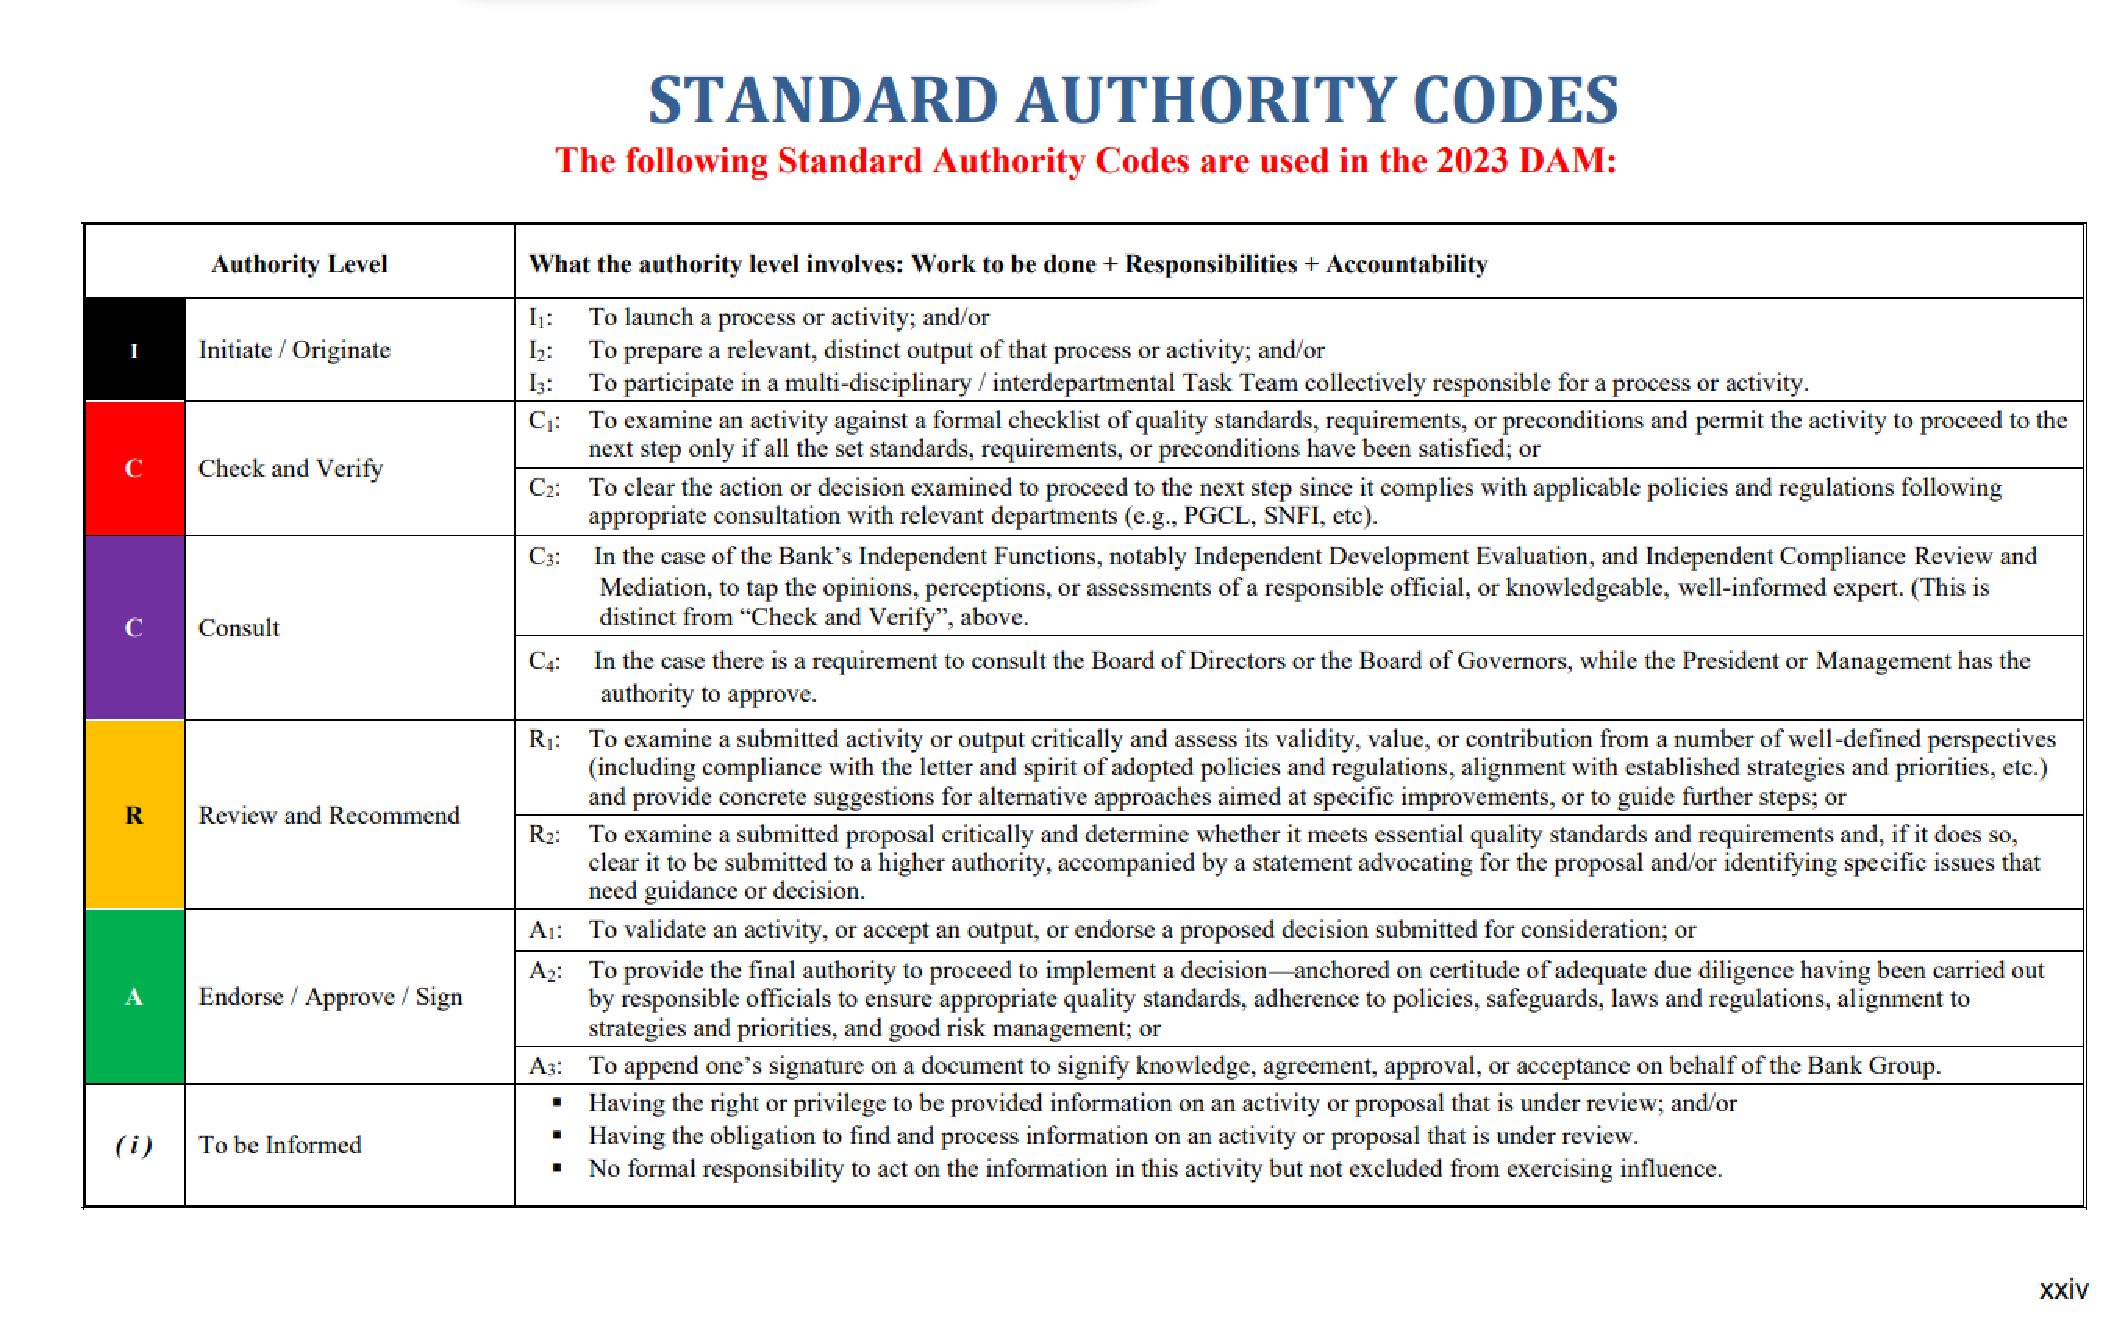
\includegraphics[width=0.88\linewidth]{figures/authority-codes.pdf}
    \caption{Authority-code legend, in which five codes expand into seventeen level-qualified notations.}
    \label{fig:authoritycodes}
\end{figure}

\subsubsection{Governance and Compliance Requirements}

The DAM is not a manual of procedures. It tells who can do something, but not how to do it. Clearly erroneous approvals would be likely to be picked up in normal organization reviews, as the individual consulted would know that it was beyond their authority. However, the DAM structure creates situations where an erroneous approval appears to be fully justified: two almost identical activities may have totally different approvers, and the person who is requested to approve is still a valid approver for this activity category as a whole — they have no way of knowing, from their position, that this particular case is assigned to someone else. This section covers the requirements that the document places on persons who wish to.This section addresses conditions for the proper interpretation of the document without any consideration of hierarchy.\\[0.3cm]
Approximation is allowed to a certain degree in most reference materials. The worst thing that can happen if an employee gets the meeting time wrong is that they miss the meeting and are able to catch up with the minutes later. This is how the DAM does not work. When a staff member misunderstands it, or misses an important role, in the course of carrying out a task, that task moves forward without the required authorisation. There is no immediate rejection or alert. The outcome is not that the reader is left without an answer, but that the reader proceeds from a self-assured but partial answer, with no hint of the opposite.\\[0.3cm]
A response can be perfectly accurate and still be misunderstood. The different tables in the DAM answer questions like “who approves X”, but by only naming the approver it conceals the need to consult others, as approval and verification are often interdependent stages of the same task – something FR4 aims to avoid. This is not an uncommon situation. Of the 216 activities that have an identified approver, 81 have no documented check or validation step. The mismatch was discovered during a trial meeting with the client – while demonstrating the agent by asking who authorises X, Yasser noticed that the response also had no check/verify function. His reasoning was that an experienced employee can easily see the connection between an approver and the person who verifies it, but a new employee may not automatically see this relationship and could easily miss it. That query showed the discrepancy, and hence the system is now giving a documented check/verification step irrespective of the initial query asked.\\[0.3cm]
Finally, the DAM file can be hard to understand for new staff without proper guidance. The staff member may miss crucial information while reading the document.
\subsubsection{Challenges in Consulting the DAM in Practice}

One of the few weaknesses of Consulting the DAM in Practice is that it takes time just to find the file in the local environment among all the other documents, and once it's found, the user still needs to scroll all the way down to the specific task that he/she needs. in some cases, even after finising it, the user can find some difficulties understanding the instruction provided by the DAM tables clearly. This causes staff to call someone more experienced to explain it.

Table~\ref{tab:twintasks} shows the problem in its sharpest form: two activities whose titles differ only in a monetary band, sitting on consecutive pages, carrying different approvers. A reader who matches on the wording alone and does not check the threshold will name the wrong approver while believing the match was exact.

\begin{table}[h]
\centering
\caption{Two near-identical activities with different approvers.}
\label{tab:twintasks}
\begin{tabular}{|l|c|p{0.4\textwidth}|l|}
\hline
\rowcolor{myblue}
\textcolor{white}{\textbf{ID}} & \textcolor{white}{\textbf{Page}} & \textcolor{white}{\textbf{Title}} & \textcolor{white}{\textbf{Approver}} \\
\hline
2.432.4.a & 43 & Individual Consultant: $\leq$ UA 50,000 & Sector Manager \\
\hline
2.433.4.c & 44 & Individual Consultant: $>$ UA 250,000 & PRC \\
\hline
\end{tabular}
\end{table}


\subsection{Study of Existing Systems}
\label{sec:existingsystems}

With the DAM's demands on readers now clear, the natural question is whether an existing tool already meets them.  We can examine two categories of tools against these weaknesses to see whether any address what the DAM lacks. The first method involves consulting the DAM and performing a manual search. The second, however, is a tool that requires using a generic question-answering assistant designed to analyze the submitted file and answer the user's question. The study of both of these systems makes it possible to better understand the needs and expectations regarding the outcome required from the DAM AI Agent.

\subsubsection{Manual Consultation and Document Search}

The current process is manual consultation of the PDF, supported by the basic search the PDF Viewer tool provides (Acrobat, Foxit,...). The Keyword search finds a character string, which helps when the staff already knows the exact title of an activity or its identifier, and helps very little otherwise. Searching for the word "approve" will return either the explanatory authority code table on the first few pages or every table in the DAM. Searching for a partially remembered activity name returns nothing at all unless the remembered words match the printed ones exactly.\\[0.3cm]

More importantly, text search returns locations not answers. It can tell the staff that a term exist in page X. It cannot tell them who approves the activity described there since that requires understanding that the pages holds a table and that the tables in the DAM have a complexe visual design and that the same action can change depending on the authority level and the footnote attached to it.

\subsubsection{Generic Document Question-Answering Assistants}

A second category of existing solustion is the General purpose document assistant tools such as ChatPDF \citep{chatpdf}, NotebookLM \citep{notebooklm} or Microsoft Copilot's file upload mode \citep{ms365copilot}. These tools typically function by splitting the document into passages, embed those passages into vectors, retrieve the passage similar to the question and then pass them to a language model that writes an answer. This is standard retrieval-augmented generation, or RAG \citep{lewis2020rag}.\\[0.3cm]
This approach performs well on the conventional text heavy documents but breaks on this document for a reason that the DAM is structural rather than literary. When a page of the DAM is converted to plain text, the spatial relationship that carry its meaning are destroyed. The rotated header that identified a column becomes a stray string lost in the extracted corpus, disconnected from the footnotes beneath it. A retrieved passage may therefore contain the activity name and the authority code letter without preserving the information that the authority code belonged to a specific cell and has a specific footnote or authority level. in that case the model is left working from a text that has already lost the answer, and produces a confident answer either ways.

\begin{figure}[htbp]
\centering
\begin{subfigure}[b]{\linewidth}
\centering
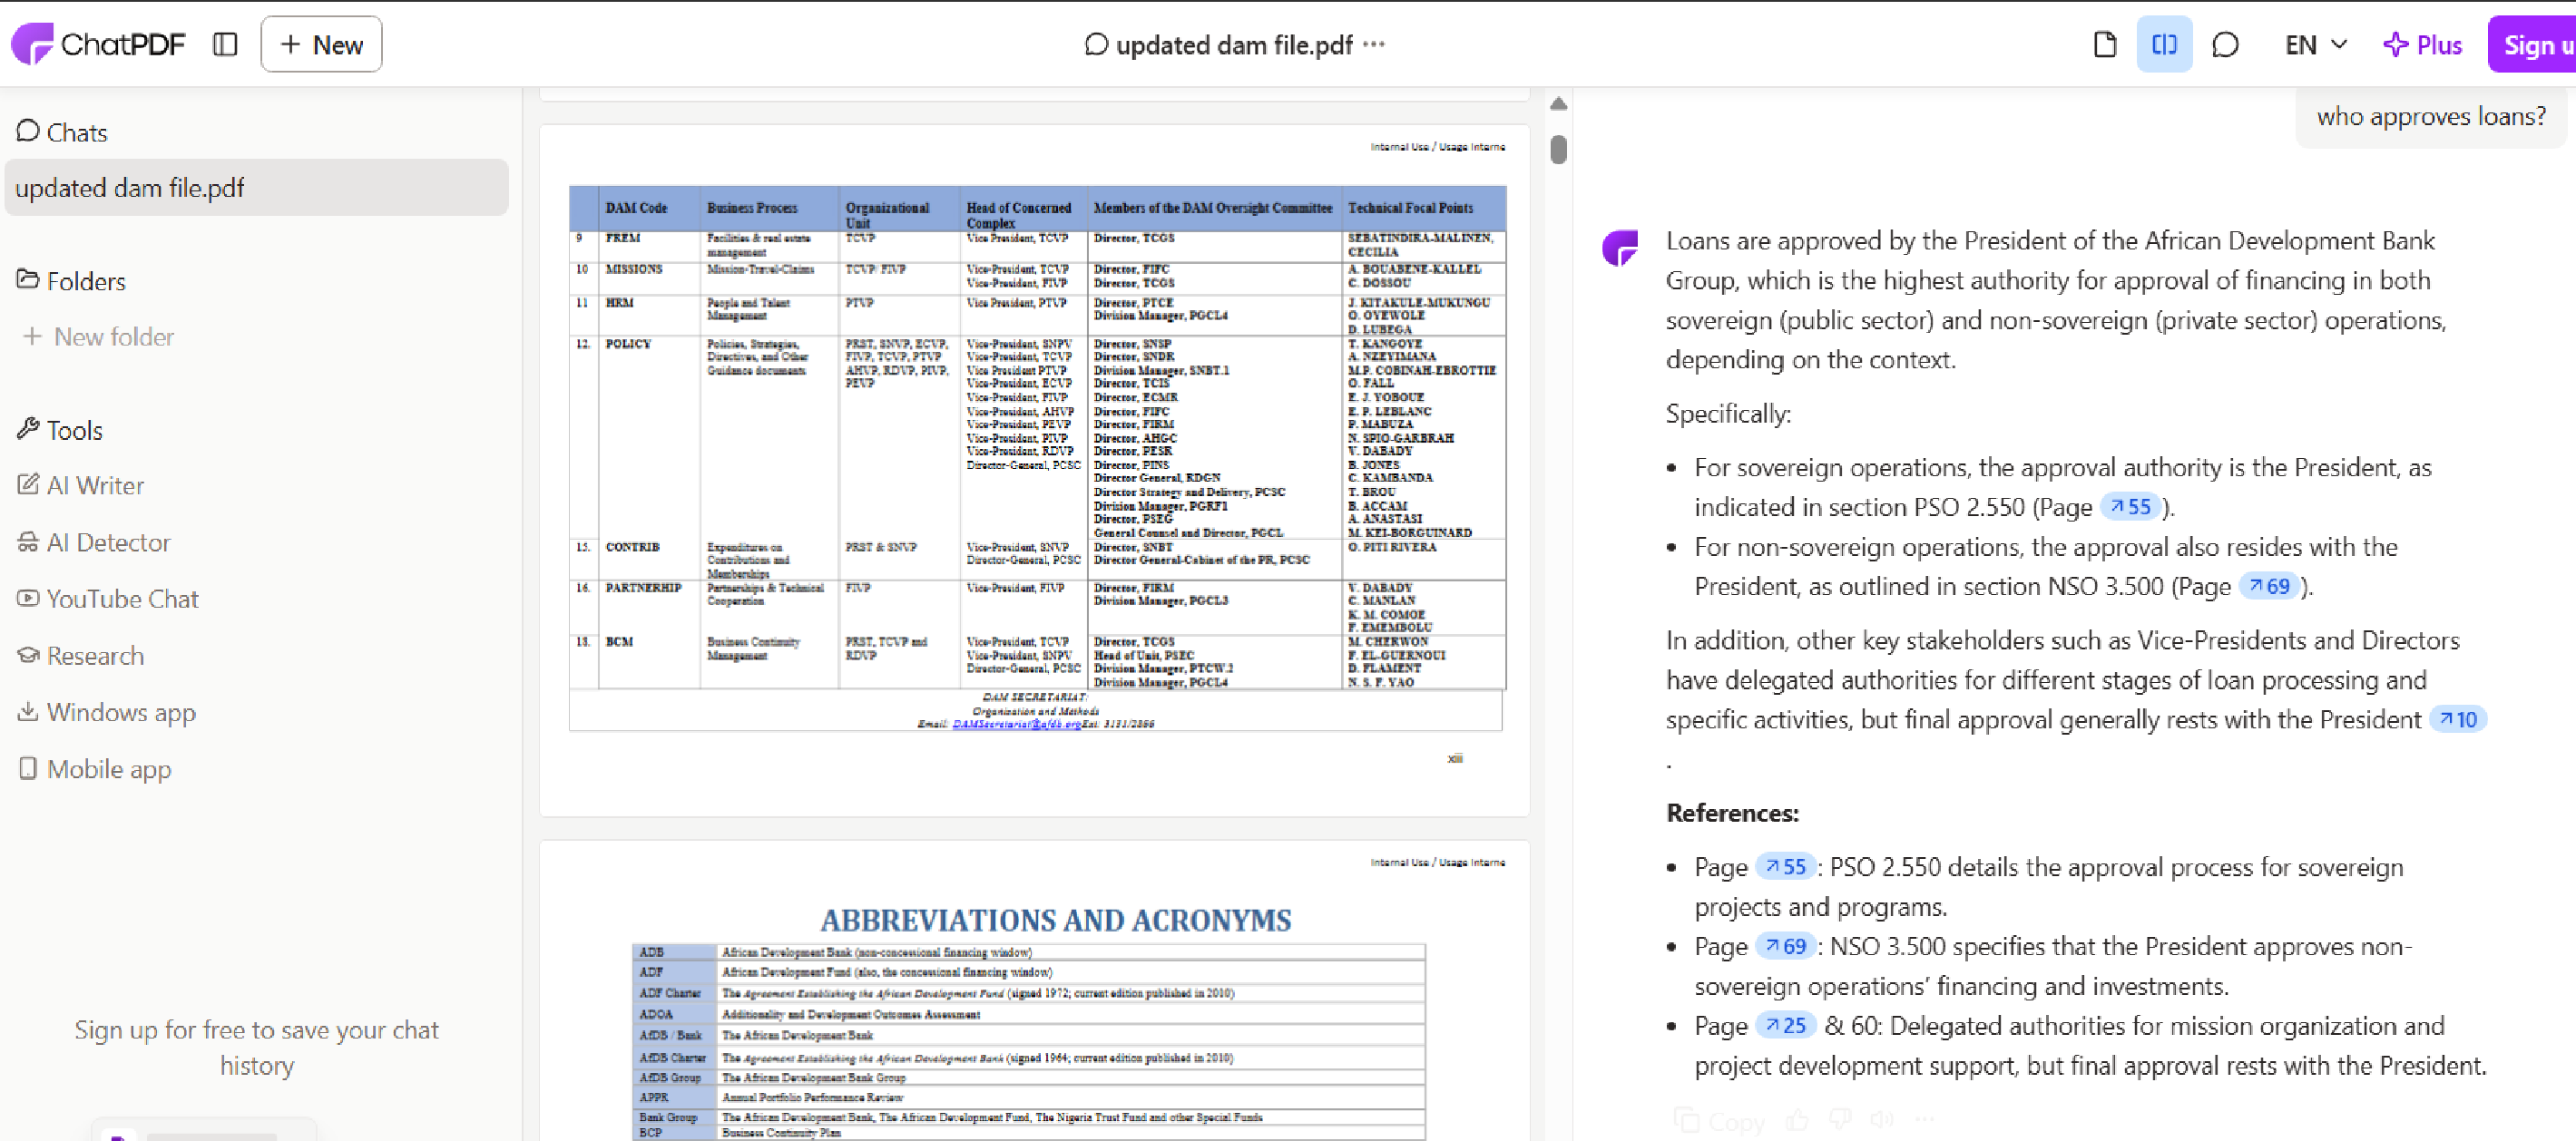
\includegraphics[width=0.92\linewidth]{figures/chatpdf-loans.pdf}
\caption{``Who approves loans?''}
\label{fig:chatpdf-loans}
\end{subfigure}
\par\bigskip
\begin{subfigure}[b]{\linewidth}
\centering
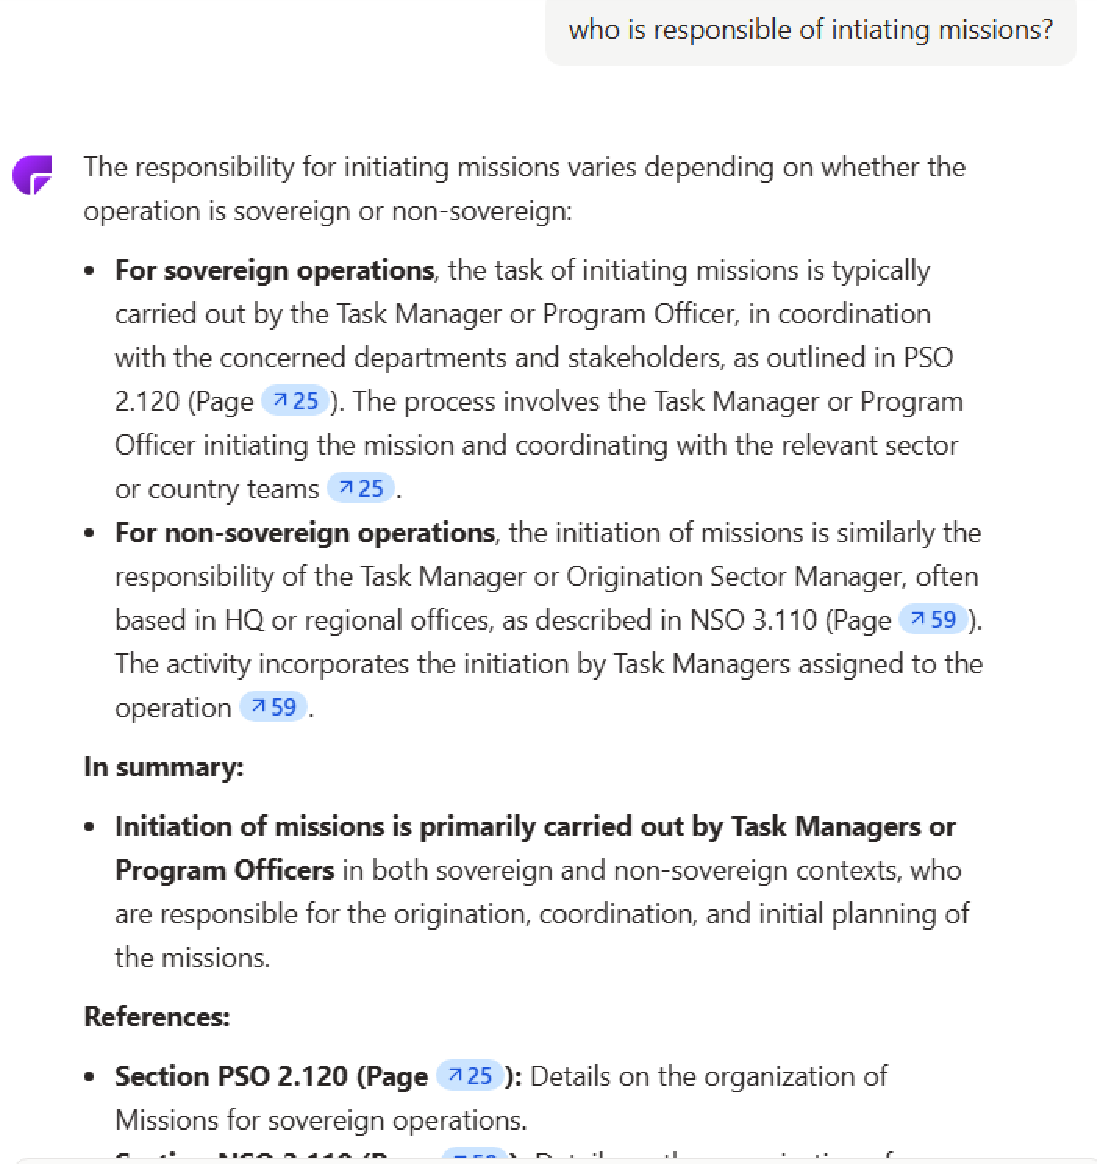
\includegraphics[width=0.92\linewidth]{figures/chatpdf-missions.pdf}
\caption{``Who is responsible for initiating missions?''}
\label{fig:chatpdf-missions}
\end{subfigure}
\caption{ChatPDF's answers to two DAM authority questions, with page citations it generated automatically. The two exchanges are stacked rather than placed side by side so that the wording of each answer stays legible at normal page width.}
\label{fig:chatpdf}
\end{figure}

To test this directly, two pages of the DAM were uploaded to ChatPDF and asked "who approves loans?" and "who is responsible for initiating missions?" (Figure~\ref{fig:chatpdf}). Both answers were fluent, well-structured, and included automatically generated page citations. Checked against this project's own extracted data, however, neither holds up at the level of detail the DAM actually records. The DAM lists the President as an approver in exactly one context — a staff-seniority escalation ladder for mission-related sign-off — not as a general final approver for loans. The specific page ChatPDF cited for loan approval in fact records a different and more complex set of roles, one of which could not even be confidently resolved to a name during this project's own extraction. The mission-initiation answer merges several distinct activities sharing a common process code into a single summary, silently dropping at least one case with a different initiator entirely. Both answers illustrate the mechanism described above: the tool produces something fluent and well-organised from a page whose spatial structure it has already discarded, and the fluency of the result gives no indication of where it has quietly generalised past what the actual row records.

\subsubsection{Critical Analysis: Limitations of Current Approaches}

Both approaches ultimately encounter a fundamental challenge: they lack an awareness of error. This is the failure mode surveyed across generative systems as hallucination\citep{ji2023hallucination}, and it is particularly consequential here, because a confidently phrased wrong approver is indistinguishable to the reader from a correct one. When a search engine produces results or a language model generates text, neither system differentiates between a supported answer and one that lacks justification. This distinction is crucial for compliance purposes.

Table~\ref{tab:existing} assesses both categories against the needs established earlier in this section, alongside the approach taken in this work.

\begin{table}[h]
\centering
\caption{Existing approaches assessed against the needs of this project.}
\label{tab:existing}
\small
\begin{tabular}{|p{0.3\textwidth}|c|c|c|c|}
\hline
\rowcolor{myblue}
\textcolor{white}{\textbf{Requirement}} &
\textcolor{white}{\textbf{Search}} &
\textcolor{white}{\textbf{Assistants}} &
\textcolor{white}{\textbf{This work}} \\
\hline
Preserves positional table meaning & No & No & Yes \\ \hline
Answers a question, not a location & No & Yes & Yes \\ \hline
Answer traceable to a source row & No & No & Yes \\ \hline
Refuses when it cannot answer & N/A & No & Yes \\ \hline
Surfaces mandatory obligations & No & No & Yes \\ \hline
Tolerates typos and loose phrasing & No & Yes & Yes \\ \hline
Document stays inside the institution & Yes & No & Yes \\ \hline
No per-page or licence cost & Yes & Partly & Yes \\ \hline
Deployable within this project & Yes & Yes & Yes \\ \hline
\end{tabular}
\end{table}

The table above presents a comparative analysis of the two existing systems for reading the DAM document. Three major differences between the systems are evident.
First, the question-answering assistant can tolerate typos within the document, whereas the manual search method does not account for such errors.
Second, the question-answering assistant differs from the manual search method by its ability to answer user questions regarding the DAM document, a capability not available with the manual search method.
Third and finally, the manual search method differs from the question-answering assistant in terms of security. Submitting an internal, confidential document of this magnitude to a generic question-answering assistant, one not created or licensed by the AFDB, constitutes a security breach. Consequently, a manual search within the document can be viewed as a less efficient but more secure solution, as it relies on no external tools that could compromise the security and confidentiality of the DAM document.\\[0.2cm]
Thus, a conclusion can be drawn from this comparative analysis of the two previously used methods. The DAM AI Agent must, first, be capable of functioning even in the presence of typos. Next, it must accurately and precisely answer the various questions a user might ask. Finally, the DAM AI Agent must comply with AFDB security standards, and the document submitted to it must remain confidential. This last point will be explained further in the Authentication section of Chapter 5.

\section{Functional Needs Analysis}

The gaps identified above translate directly into requirements: each one traces back to a
specific limitation of manual search or generic assistants documented in the preceding
section.

\subsection{Functional requirements}

The functional requirements are categorised into two groups. Requirements FR1 to FR10 pertain to the fundamental question-answering capability and derive from current document consultation practices. Requirements FR11 to FR15 address the platform capabilities introduced in the project's second phase, which transform the system from a lookup tool into an application usable inside an institution. Table~\ref{tab:fr} describes each of them.

Every requirement listed satisfies two conditions. It corresponds to a need observed in the way the document is consulted, rather than to a capability that merely seemed attractive to build; and it is met by the delivered system. Requirements that failed either condition were removed rather than retained as statements of intent, since a requirements table describing intentions cannot be used to evaluate what was actually produced.

\begin{longtable}{|p{0.08\textwidth}|p{0.26\textwidth}|p{0.54\textwidth}|}
\caption{Functional requirements.}\label{tab:fr}\\
\hline
\rowcolor{myblue}\textcolor{white}{\textbf{Ref.}} & \textcolor{white}{\textbf{Requirement}} & \textcolor{white}{\textbf{Description}} \\
\hline
\endfirsthead
\hline
\rowcolor{myblue}\textcolor{white}{\textbf{Ref.}} & \textcolor{white}{\textbf{Requirement}} & \textcolor{white}{\textbf{Description}} \\
\hline
\endhead
FR1 & Direct identifier lookup & Given a valid activity identifier, the system returns that activity's recorded authority information with full confidence and no ambiguity. \\ \hline
FR2 & Natural-language lookup & Given a question describing an activity by name rather than by identifier, the system resolves it to the correct activity and reports how confident that resolution is. \\ \hline
FR3 & Authority-role queries & For a resolved activity, the system answers who approves, reviews, checks, initiates, or must be informed, using the document's own notation. \\ \hline
FR4 & Mandatory obligation surfacing & Whatever the question asked, the system always surfaces a recorded check-and-verify obligation and, where present, the informed parties. \\ \hline
FR5 & Cross-reference resolution & Where an activity's row is a pointer to another activity, the system follows the pointer automatically rather than reporting that no responsibilities exist. \\ \hline
FR6 & Typing and phrasing tolerance & The system tolerates common misspellings and phrasing variation without requiring the document's exact vocabulary. \\ \hline
FR7 & Honest refusal & For an identifier that does not exist, or a question outside the document's subject matter, the system says so explicitly instead of returning a best guess. \\ \hline
FR8 & Conversational continuity & A follow-up question that does not restate its subject is answered against the activity discussed immediately before. \\ \hline
FR9 & Structural analytics & The system exposes an overview of the document's own structure: node counts, authority-code distribution, roles most frequently involved, and per-chapter breakdowns. \\ \hline
FR10 & Multilingual questions & Questions asked in French, Spanish, Portuguese, or Arabic are answered in the language they were asked in, without translating role names or identifiers. \\ \hline
FR11 & Authenticated access & Access to the application requires authentication, and analytical features are restricted to authorised roles. \\ \hline
FR12 & Voice input & A user can dictate a question instead of typing it, in any of the supported interface languages. \\ \hline
FR13 & Document attachment & A user can attach a supporting document to a conversation and ask questions about its content, with answers from that source clearly distinguished from answers grounded in the DAM. \\ \hline
FR14 & Localised conversation interface & The conversation interface, including its controls and its answer provenance labels, is available in each supported language, with right-to-left layout applied for Arabic. \\ \hline
FR15 & Conversation sharing & A user can grant a colleague read-only access to a conversation, either by naming them directly or through an expiring link encoded as a QR code, with shared views reflecting new messages without requiring a page reload. \\ \hline
\end{longtable}

\subsection{Non-Functional Requirements}

Where the functional requirements state what the system must do, the non-functional requirements state the qualities it must exhibit while doing it. They are not secondary. NFR1 in particular, which forbids any answer from naming a role or code the source document does not record for that activity, takes precedence over fluency, latency, and every other consideration in the table: a system of this kind that is pleasant to use and occasionally wrong is worse than no system at all, because it transfers confidence without transferring correctness. The remaining requirements span traceability, availability, reproducibility, portability, and the handling of credentials and uploaded files. Table~\ref{tab:nfr} details each one.

\begin{longtable}{|p{0.08\textwidth}|p{0.26\textwidth}|p{0.54\textwidth}|}
\caption{Non-functional requirements.}\label{tab:nfr}\\
\hline
\rowcolor{myblue}\textcolor{white}{\textbf{Ref.}} & \textcolor{white}{\textbf{Requirement}} & \textcolor{white}{\textbf{Description}} \\
\hline
\endfirsthead
\hline
\rowcolor{myblue}\textcolor{white}{\textbf{Ref.}} & \textcolor{white}{\textbf{Requirement}} & \textcolor{white}{\textbf{Description}} \\
\hline
\endhead
NFR1 & Factual fidelity & No answer may contain a role, code, or qualification that is not recorded in the source document for that activity. This requirement takes precedence over fluency, speed, and every other consideration. \\ \hline
NFR2 & Traceability & Every answer must be attributable to a specific activity record so that a user can verify it against the printed document. \\ \hline
NFR3 & Availability without external services & Core lookup must work when no language model provider is reachable, degrading to template answers rather than failing. \\ \hline
NFR4 & Response time & Answers should return within a few seconds on the free hosting tier used for deployment, which rules out re-parsing the document per request. \\ \hline
NFR5 & Reproducibility & The same question must produce the same underlying facts on every run, independent of any model's sampling behaviour. \\ \hline
NFR6 & Portability & The system must run identically on a developer machine and on the hosting platform, without environment-specific configuration. \\ \hline
NFR7 & Usability on any device & The interface must remain usable on a phone, since consultation often happens away from a desk. \\ \hline
NFR8 & Credential protection & Authentication credentials must never be stored in recoverable form, and session tokens must expire. \\ \hline
NFR9 & Upload safety & Attached documents must be constrained by type and size, and must never be executed or interpreted as anything other than text to be read. \\ \hline
\end{longtable}

\subsection{Project Constraints}

The conditions below were fixed before any design decision was taken, and each one closed off an approach that would otherwise have been reasonable. They are recorded here because several choices defended later in this report, particularly the preference for lexical retrieval over learned embeddings and the decision to cache the parsed knowledge base at build time, follow directly from them rather than from a free comparison of alternatives. Table~\ref{tab:constraints} sets out each constraint and what it ruled out.

\begin{longtable}{|p{0.30\textwidth}|p{0.58\textwidth}|}
\caption{Project constraints.}\label{tab:constraints}\\
\hline
\rowcolor{myblue}\textcolor{white}{\textbf{Constraint}} & \textcolor{white}{\textbf{Consequence for the project}} \\
\hline
\endfirsthead
\hline
\rowcolor{myblue}\textcolor{white}{\textbf{Constraint}} & \textcolor{white}{\textbf{Consequence for the project}} \\
\hline
\endhead
No labelled training data & No query-and-answer pairs and no annotated tables existed, which ruled out training a supervised model and pushed retrieval toward lexical methods that need no training corpus. \\ \hline
Document scope & The full DAM exceeds 250 pages. Work was scoped to a 79-page subset covering three chapters, with the remainder left as future work. \\ \hline
No infrastructure budget & Deployment had to fit within free hosting tiers, which constrained memory use and forced the parsed knowledge base to be cached at build time rather than rebuilt on startup. \\ \hline
Verification against the source & Because no ground-truth dataset existed, correctness had to be established by comparison against real pages of the document, which set the pace of the data understanding phase. \\ \hline
\end{longtable}

\section{Proposed Solution}

The requirements above rule out both alternatives surveyed earlier: manual search cannot
answer a question, and a generic assistant cannot be trusted to answer it correctly. The
system described in the rest of this chapter is built to do both, starting from a general
design principle and then the four-layer architecture that implements it.

\subsection{General Presentation of the Solution}

The proposed system delineates two distinct tasks that conventional assistants typically merge: ascertaining factual content and determining the appropriate manner of expression. The factual information is extracted from a structured knowledge base, created by analyzing the document once offline, utilizing rules derived from the document’s own structure and subsequently validated against printed materials. In contrast, phrasing is managed by a language model, which rewords facts that have been previously retrieved.

In between these two layers, a crucial verification process occurs. Before any generated response is presented to the user, it undergoes a comparison with the retrieved facts. Any response that omits or modifies a role name is discarded in favor of a predetermined template. Consequently, users receive accurate answers, albeit delivered in a less conversational format. This verification mechanism ensures the language model's safe application within this context. It is described in detail in Chapter~4.

\subsection{Global System Architecture}

The system comprises four distinct layers. The offline extraction layer converts the source PDF into a validated set of nodes, which are subsequently cached and included with the application. The knowledge layer utilizes this node set as a directed graph, enabling efficient searches and lookups. The agent layer interprets user inquiries, translates them into actionable tasks, formulates definitive responses, and utilizes the language model along with a verification process. Finally, the presentation layer interfaces with the agent through a REST framework, facilitating conversation, document attachment, export, sharing, and analytics features.

Figure~\ref{fig:architecture} shows how these four layers relate, and in particular where the boundary between offline and online work falls.

\begin{figure}[htbp]
\centering
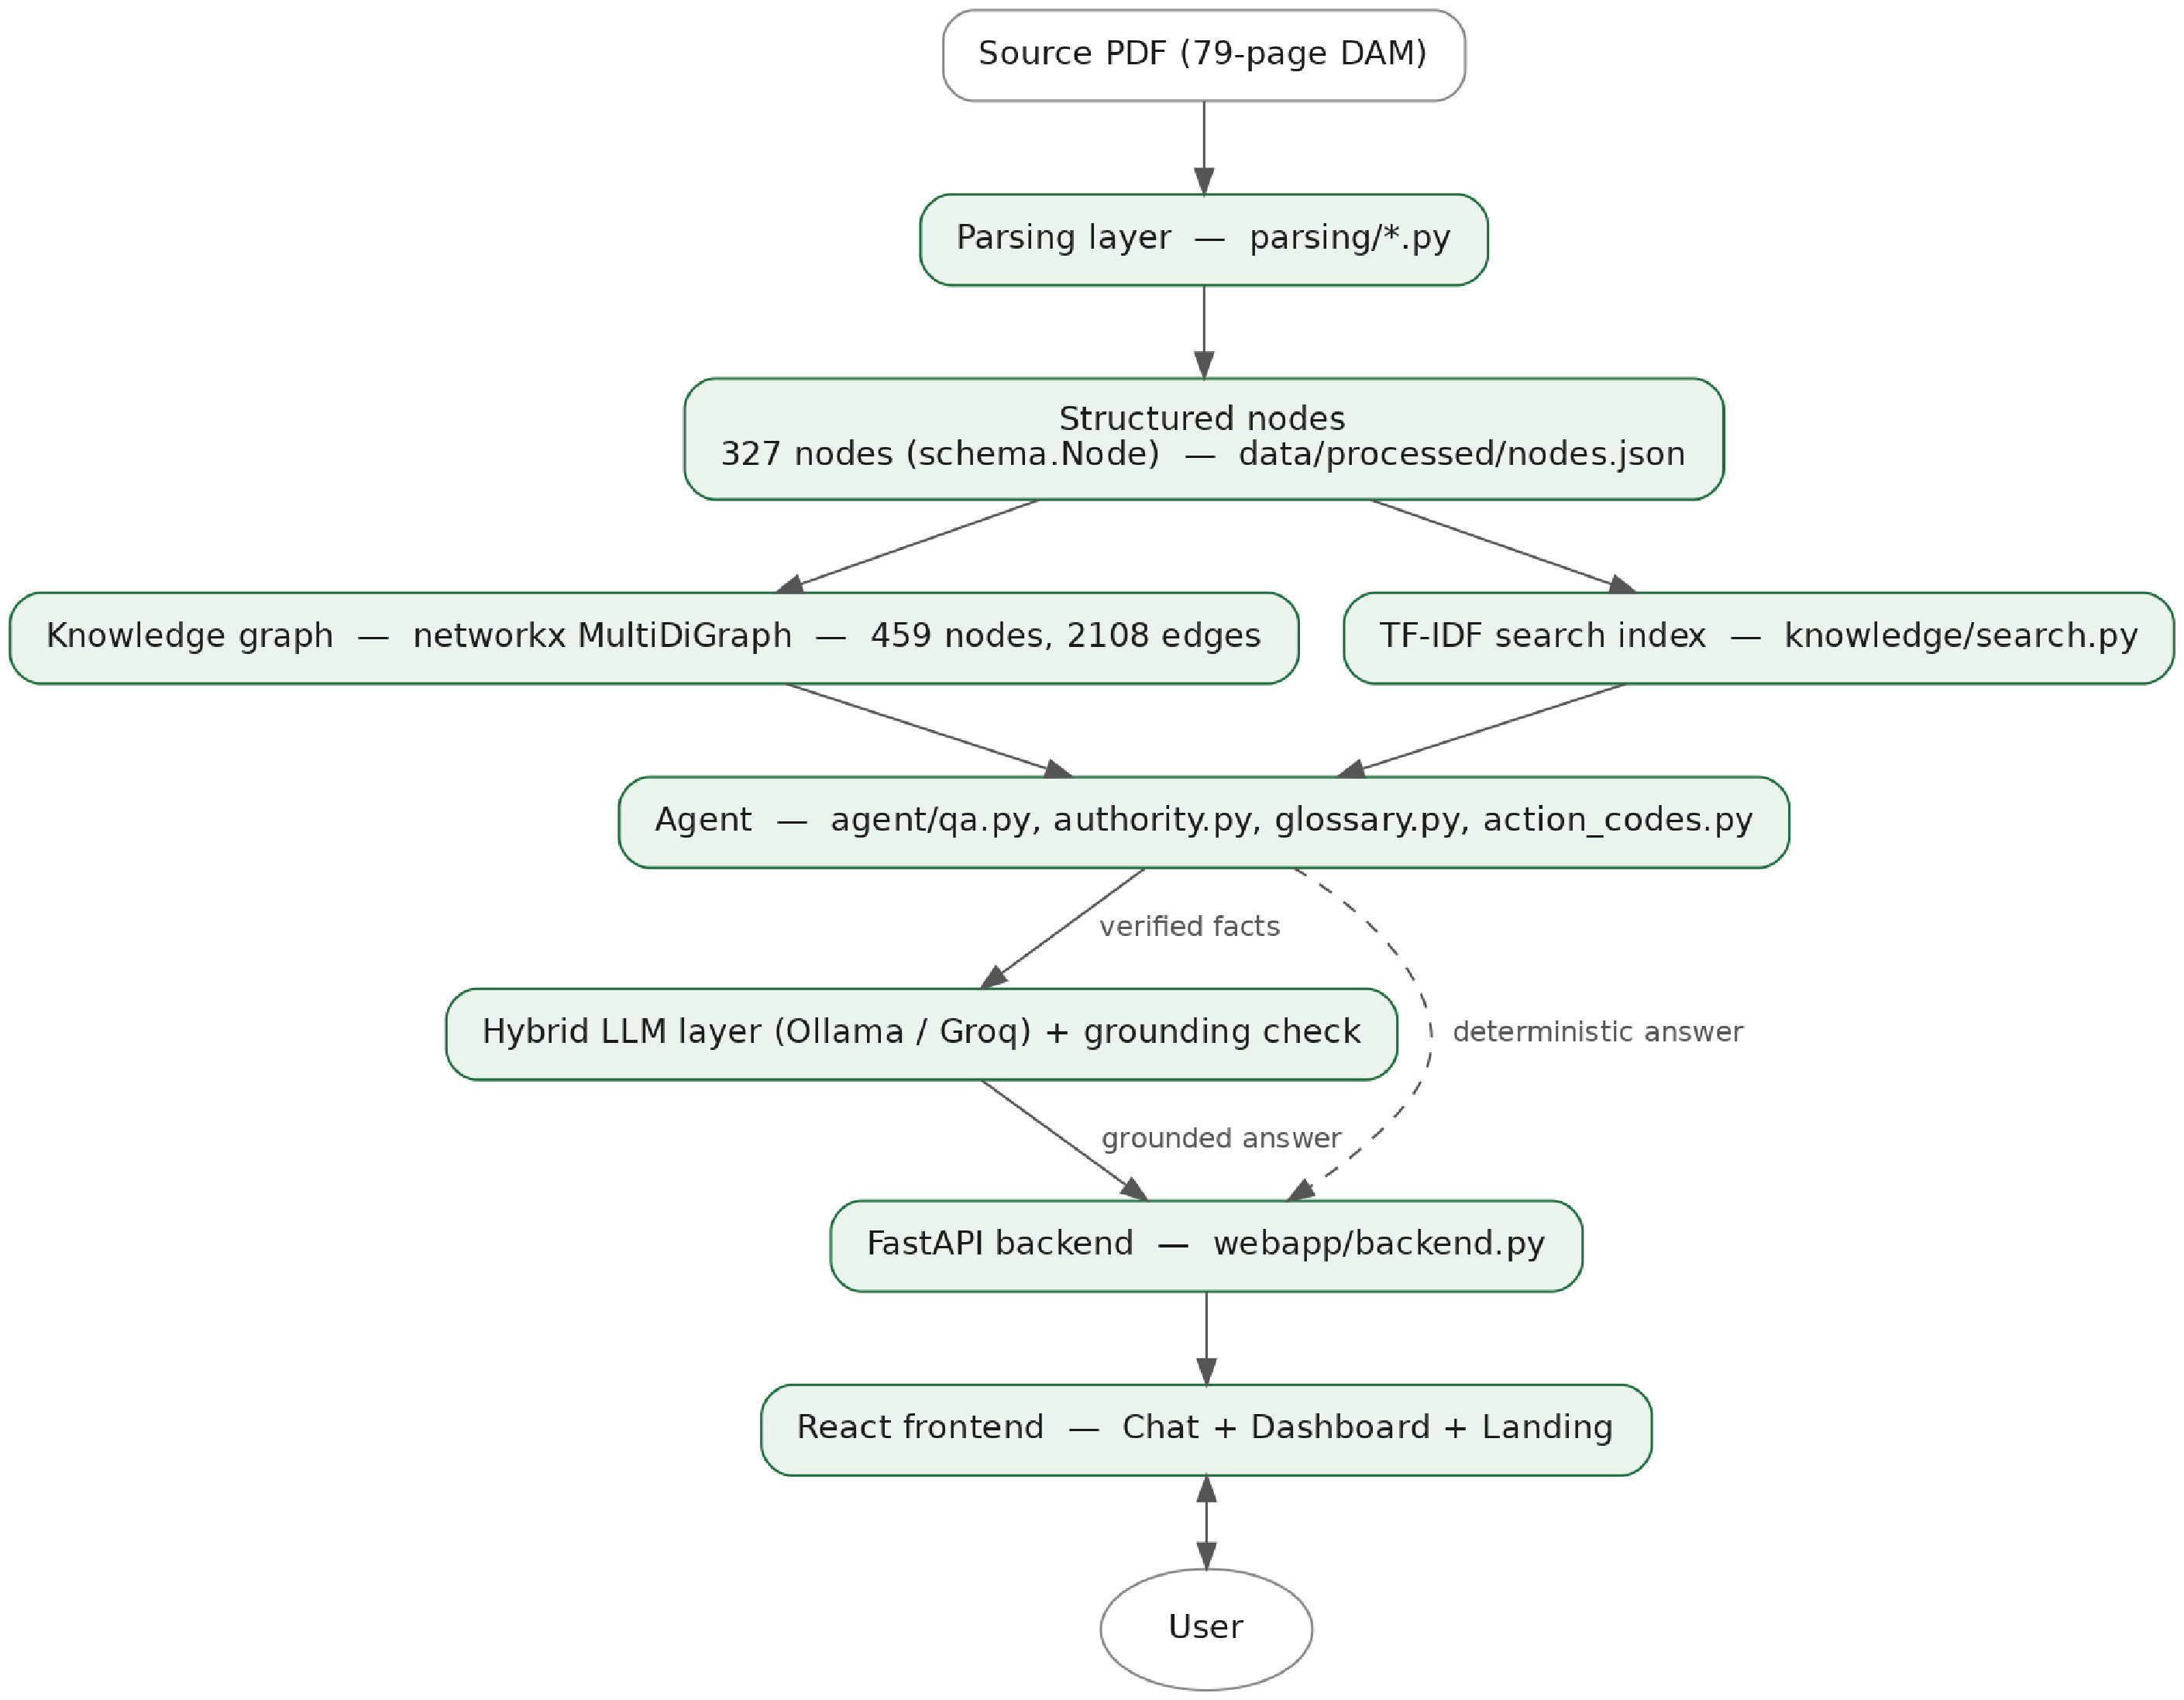
\includegraphics[width=0.94\textwidth,height=0.88\textheight,keepaspectratio]{figures/fig1_architecture.pdf}
\caption{Global architecture of the proposed system, from source document to user-facing answer.}
\label{fig:architecture}
\end{figure}

One notable consequence of this separation is that, because extraction occurs offline and its output is cached, the running application interacts exclusively with a prepared set of nodes stored in memory at startup, never directly accessing the PDF. This approach was adopted for deployment efficiency,

\subsection{Selected Technologies}

Several tools and technologies were selected to serve a specific purpose in the construction of the system, and each was chosen against the constraints recorded in Table~\ref{tab:constraints} rather than on general merit. Table~\ref{tab:tech} lists each technology and the role it plays.

\begin{longtable}{|p{0.26\textwidth}|p{0.62\textwidth}|}
\caption{Selected technologies and their role in the system.}\label{tab:tech}\\
\hline
\rowcolor{myblue}\textcolor{white}{\textbf{Technology}} & \textcolor{white}{\textbf{Role in the system}} \\
\hline
\endfirsthead
\hline
\rowcolor{myblue}\textcolor{white}{\textbf{Technology}} & \textcolor{white}{\textbf{Role in the system}} \\
\hline
\endhead
Python & Language for extraction, knowledge base, agent, and backend. \\ \hline
pdfplumber\citep{pdfplumber} & Character- and word-level PDF extraction with positional coordinates, which is what makes geometric reasoning about rotated headers and superscripts possible. \\ \hline
Pydantic\citep{pydantic_docs} & Schema definition and validation for the node model, so malformed records fail at construction rather than at query time. \\ \hline
networkx\citep{hagberg2008networkx} & Knowledge graph construction and traversal, using a directed multigraph so that a role can hold several distinct responsibilities over the same activity. \\ \hline
scikit-learn\citep{pedregosa2011sklearn} & TF-IDF vectorisation and cosine similarity for free-text activity resolution. \\ \hline
FastAPI\citep{fastapi_docs} & REST backend, chosen for its typed request and response models and automatic API documentation. \\ \hline
React\citep{react_docs} and Vite\citep{vite_docs} & Web client, built as four independent per-page bundles rather than a single-page application, and served as pre-built static files by the backend. \\ \hline
Groq\citep{groq} and Ollama\citep{ollama} & Language model providers for answer phrasing, cloud-hosted and local respectively, behind a common interface so either can be used or neither. \\ \hline
Whisper (hosted)\citep{groq} & Server-side transcription of dictated questions, chosen over browser speech recognition for consistent behaviour across clients. \\ \hline
Web Speech API\citep{webspeech_api} & Browser-native speech synthesis for reading answers aloud, which keeps audio playback entirely on the client. \\ \hline
python-jose\citep{python_jose_docs} and passlib\citep{passlib_docs} & JSON Web Token issuing and password hashing for the authentication layer. \\ \hline
Docker\citep{docker_docs} & Containerisation, so the application runs identically in development and in deployment. \\ \hline
Render\citep{render_docs} & Hosting platform, used on its free tier. \\ \hline
\end{longtable}

\section*{Conclusion}
\addcontentsline{toc}{section}{Conclusion}

The Document Asset Management (DAM) system addresses a critical issue, yet its publication format significantly hinders accessibility. Manual consultation proves to be both slow and susceptible to error due to the document's meaning being intricately linked to its layout. Similarly, generic document assistants encounter challenges for the same reason, often resulting in a lack of fluency. The aforementioned requirements aim to address these issues, and the proposed architecture effectively separates factual retrieval from wording. This approach harnesses the potential of language models while mitigating their inherent unreliability. The subsequent chapter will delve into the source document, exploring the complexities involved in its extraction.
